\documentclass[tikz, border = 10pt]{standalone}

%%%<
\usepackage{verbatim}
\usetikzlibrary{calc, intersections, through}
%%%>

\begin{comment}
:Title: Ramanujan's Construction of 355/113, an approximation to pi
:Author: Moti Ben-Ari
:Tags: Geometry;Intersections;Straightedge and compass;pi
:Slug: Ramanujan's approximation to pi

TikZ features: name path, name intersections, circle through,
  partway modifier, veclen, let..in


  With a straightedge and compass it is possible to construct
  any real number that can be obtained from the integers
  using the four arithmetic operators +, -, *, / and square roots.
  Only these numbers can be constructed. See, for example:
    John B. Fraleigh. _A First Course in Abstract Algebra,
    7th Edition_, Pearson, 2003, Section 32.
  Therefore, the value of pi cannot be constructed
  because pi is a transcendental number.
  
  There are approximations to pi such as 355/113 = 3.14159292,
  which differs from pi only in the seventh decimal place.
  Computing the circumference of the earth from its diameter,
  using 355/113 instead of pi gives an error of less than 4 meters!
  
  A naive construction of 355/113 would take hundreds of steps.
  Ramanujan found a clever construction that requires
  only 12 line segments.
    The Journal of the Indian Mathematical Society, 1913, p. 138.
    https://en.wikisource.org/wiki/Squaring_the_circle.

  This examples gives Ramanujan's construction.
  
  Ramanujan (1887--1920) grew up in southern India and quickly
  advanced beyond the mathematical level of local colleges.
  He sent his work to G.H. Hardy who invited him to England.
  Ramanujan arrived in 1914 but could not return home
  until after World War I.
  He suffered from the cold climate and from the difficulty of
  adhering to a strict vegetarian diet.
  Ramanujan died at age 32 shortly after returning to India.
  His mathematics is still the subject of research.
    Robert Kanigel. _The Man Who Knew Infinity:
    A Life of the Genius Ramanujan_, Schribner's, 1991.
  
    Construction

      1. The construction follows the one by Ramanujan.
         Occasionally, TikZ's calc library is used for brevity
         instead of the full construction, for example,
         to bisect a line segment.

      2. Each line segment will be labeled with its length.
         Only the outline of a composition is given;
         for details see:
         "Surprising constructions with straightedge and compass"
         https://www.weizmann.ac.il/sci-tea/benari/mathematics).
\end{comment}

\begin{document}

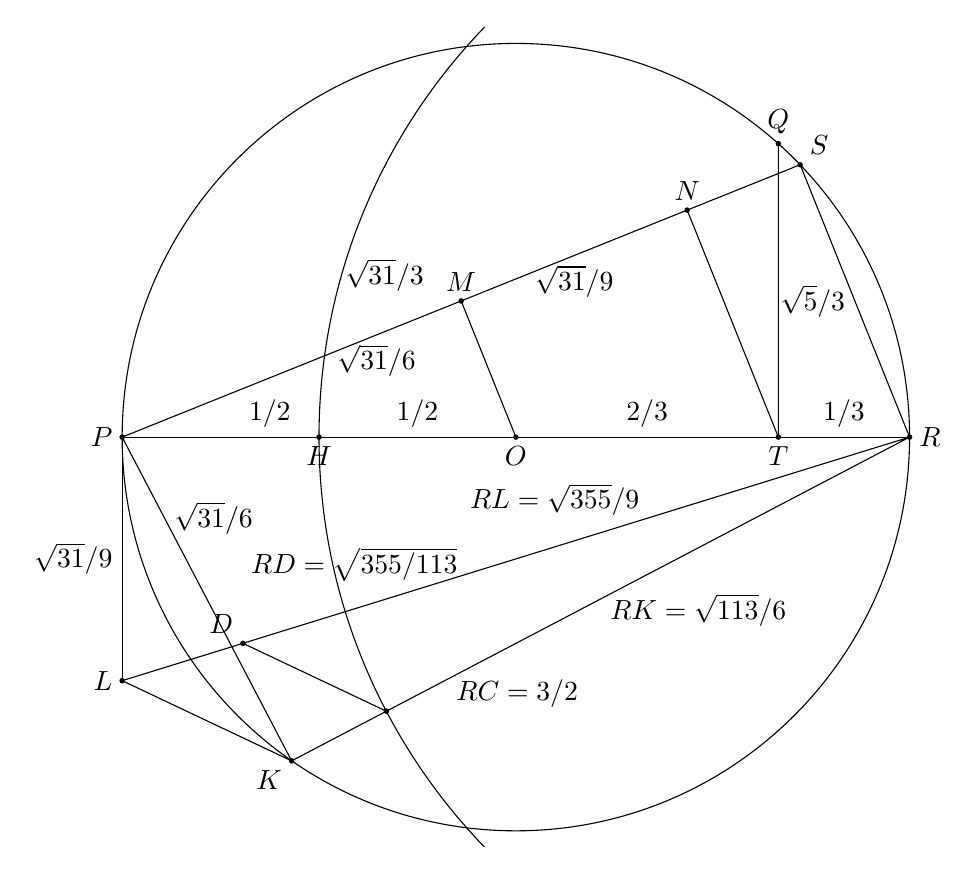
\begin{tikzpicture}

  % Clip the picture to its actual size.
  
  \clip (-6.2, -5.2) rectangle (5.5, 5.2);
  
  % Construct a line segment which will be the diameter of
  %   the unit circle.
  % Label its endpoints P, R and its midpoint O.
  % For clarity, the diameter is drawn with a length of 10 cm.
  
  \draw (-5, 0) coordinate (P) node[left]  {$P$} --
        ( 5, 0) coordinate (R) node[right] {$R$};
  \coordinate[label = below:$O$] (O) at (0, 0);
  \fill (P) circle(1pt);
  \fill (O) circle(1pt);
  \fill (R) circle(1pt);
  
  % Use circle through to draw a "unit" circle centered at O.
  
  \node [draw, name path = circle] at (O)
    [circle through = (P)] {};
  
  % Bisect PO (using the partway modifier) and label the midpoint H.
  % Label the lengths of PH and HO.
  
  \coordinate[label = below:$H$] (H) at ($ (P) ! .5 ! (O) $);
  \fill (H) circle(1pt);
  \path (P) -- node[above, near end] {$1/2$} (H);
  \path (H) -- node[above] {$1/2$} (O);
  
  % Trisect the radius OR and label the point 2/3 from O by T.
  % (Trisecting a _line segment_ means multiply it by the rational
  % number 1/3. What is impossible is to trisect and angle!)
  % Label the lengths of OT and TR.
  
  \coordinate[label = below:$T$] (T) at ($ (O) ! .6667 ! (R) $);
  \fill (T) circle(1pt);
  \path (O) -- node[above] {$2/3$} (T);
  \path (T) -- node[above] {$1/3$} (R);
  
  % Construct a perpendicular to OR at T and label its
  %   intersection with the circle Q.
  
  % Method:
  %   First \draw a perpendicular from T and ensure that it
  %     is long enough to intersect the circle.
  %   The path is drawn using |- to take the x-coordinate as
  %     the x-coordinate of T and the y-coordinate as 5 cm
  %     above T.
  %   Get the point of intersection Q.
  %   Replace the \draw of the perpendicular by \path
  %     so that it is invisible and just \draw QT.

  \path [name path = QT] (T) |- +(0, 5);
  \path [name intersections = {% % The comment is necessary!
     of = QT and circle,
     by = Q
     }];
  \fill (Q) circle(1pt);
  \draw (T) -- (Q) node[above] {$Q$};
  
  % Construct a chord from R of length QT which intersects
  %   the circle at S
  
  % Method:
  %   Use veclen to get the length of QT and draw a circle
  %     centered at R with this radius.
  %   S is one of the intersections of this circle with 
  %     the unit circle.
  
  \path[name path = RScircle] (R)
    let
      \p1 = ($(T) - (Q)$)
    in 
      circle ({veclen(\x1, \y1)});

  \path[name intersections = {% % The comment is necessary!
    of = RScircle and circle,
    by = S
    }];
  \fill (S) circle (1pt);
  
  % Computation:
  %   QOT is a right triangle since QT is perpendicular to PR.
  %   OQ is 1, the radius of the unit circle.
  %   OT is 2/3 by construction.
  %   The length of QT is obtained from Pythagoras's theorem.
  
  \draw (R) -- node[left] {$\sqrt{5}/3$} (S)
    node[above right] {$S$};
  
  % Draw the line segment PS.

  \draw[name path = PS] (P) -- (S);
  
  %  Computation:
  %    PSR is a right triangle since angle PSR
  %    subtends a diameter. PR is 2, the diameter
  %    of the unit circle and SR = QT which we just computed.
  %    The length of PS is obtained from Pythagoras's theorem.
  
  %  Note: the label could have been added to the previous command
  %   which draws PS but for clarity a separate \path is used.
  
  \path (P) -- node[above left, xshift = -10pt] {$\sqrt{31}/3$} (S);
  
  % Find the point N on PS such that TN is parallel to SR.
  
  % Method:
  %   In the triangle PSR, the length of any line segment parallel
  %   to SR and closer to P than SR will be shorter than SR,
  %   so a line of length S-R from T will necessarily intersect PS.
  
  \path[name path = TN] (T) -- +($(S) - (R)$);
  \path[name intersections = {% % The comment is necessary!
    of = PS and TN,
    by = N
    }];
  \fill (N) circle (1pt);
  \draw (T) -- (N) node[above] {$N$};
  
  % Find the point M on PS such that OM is parallel to SR.
  
  % Method: as for N
  
  \path[name path = OM] (O) -- +($(S) - (R)$);
  \path[name intersections = {% % The comment is necessary!
    of = PS and OM,
    by = M
    }];
  \draw (O) -- (M) node[above] {$M$};
  \fill (M) circle (1pt);
  
  % Computation:
  %   By similar triangles PM / PO = PS / PR.
  %   PM can be computed from PO, PS, PR whose lengths are known.
  
  \path (P) -- node[below, near end] {$\sqrt{31}/6$} (M);
  
  % Computation:
  %   By similar triangles PN / PT = PS / PR.
  %   PN can be computed from PT, PS, PR whose lengths are known.
  %   MN = PN - PM.
  
  \path (M) -- node[below] {$\sqrt{31}/9$} (N);
  
  % Construct the chord PK such that PK = PM.
  
  % Method:
  %   Draw a circle with center P and radius PM.
  %   It will intersect the unit circle at two points.
  %   Experimentally, determine that the required intersection 
  %   of the two circles is the second one.
  
  \node [name path = PKcircle] at (P)
    [circle through = (M)] {};
  \path[name intersections = {% % The comment is necessary!
    of = PKcircle and circle,
    by = {dummy, K}
    }];
  \fill (K) circle(1pt);
  
  % The length of PK equals the known length of PM.
  
  \draw (P) -- node[right, near start] {$\sqrt{31}/6$} (K)
    node[below left] {$K$};
  
  % Construct a tangent PL to P of length MN.

  % Method:
  %   A tangent is at right angles to a radius.
  %   Since PR is horizontal we just need a vertical line
  %     segment from P.
  %   Use the length of MN in a coordinate calculation.
  %   The length is multiplied by a factor of 5 since the picture
  %   is 5 times larger than the construction.

  \draw (P) --
    node[left] {$\sqrt{31}/9$}
    +($ {5 * sqrt(31) / 9}*(0, -1) $) coordinate (L)
    node[left] {$L$};
  \fill (L) circle(1pt);
  
  % Draw the sides of the triangle LKR which also displays the
  %   triangle PLR.
  
  \draw (L) -- (K) -- (R) -- cycle;
  
  % Computation:
  %   PKR is a right triangle because it subtends a diameter.
  %   PR is 2, the length of the diameter.
  %   The length of PK has been computed.
  %   The length of RK is obtained from Pythagoras's theorem.
  
  \path[name path=RK] (R) --
    node[right, yshift = -4pt]
    {$RK=\sqrt{113}/6$} (K);
  
  % Computation:
  %   PLR is a right triangle because PL is a tangent.
  %   PR is 2, the length of the diameter.
  %   The length of PL has been computed.
  %   The length of RL is obtained from Pythagoras's theorem.
  
  \path[name path = RL] (R) --
    node[above, xshift = 14pt, yshift = 12pt]
    {$RL = \sqrt{355}/9$} (L);
  
  % Construct C on RK such that RC = RH.

  % Method:
  %   Draw a circle at R through H and find its intersection
  %   with RK.

  \node [draw, name path = RHcircle] at (R)
    [circle through = (H)] {};
  \path [name intersections = {% % The comment is necessary!
     of = RK and RHcircle,
     by = C
     }];
  \fill (C) circle (1pt);
  
  % RC = RH so the length of RC is 3/2.

  \path (R) -- node[below, near end, yshift = -10pt]
    {$RC = 3/2$} (C);
  
  % Construct D such that CD is parallel to LK.
  
  % Method
  %   L-K is a vector pointing in the same direction as LK.
  %   Draw a line segment in this direction from C.
  %   Its intersection with RL gives the required point D.

  \path[name path = CD] (C) -- +($ (L) - (K) $);
  \path[name intersections = {% % The comment is necessary!
    of = CD and RL,
    by = D
    }];
  \fill (D) circle (1pt);
  \draw (C) -- (D) node[above left] {$D$};
  
  % Computation:
  %   Since CD is parallel to LK, by similar triangles,
  %   RD / RC = RL / RK.
  %   RD can be computed from RC, RL, RK whose lengths are known.
  
  \path (R) --
    node[above, near end, xshift = -20pt]
    {$RD=\sqrt{355/113}$} (D);
  
  % Square the length of RD to obtain 355/113.
  % The construction is easy and is omitted.

\end{tikzpicture}

\end{document}
